\documentclass{article}

\usepackage{tikz}
\usetikzlibrary{arrows, bending}
\usetikzlibrary{arrows.meta}
\begin{document}
\pagestyle{empty}
% \section*{100 res}

% \begin{tikzpicture}
%     % \draw[help lines] (0,0) grid (5,5)

%     \node (NK_X1)  [draw, circle] at (1,9) {NK\_X1};
%     \node (SP_Y1)  [draw, circle] at (3,5) {SP\_Y1};
%     \node (BO_X2)  [draw, circle] at (1,1) {BO\_X2};
%     \node (KP_Y2)  [draw, circle] at (9,5) {KP\_Y2};


%     \node (X21) [draw, rectangle, left of=BO_X2, xshift=-1cm,yshift=1cm] {X21};
%     \node (X22) [draw, rectangle, below of=X21] {X22};
%     \node (X23) [draw, rectangle, below of=X22] {X23};
%     \node (X24) [draw, rectangle, below of=X23] {X24};

%     \draw [-{Latex[length=3mm]}] (BO_X2) -- node[above] {0.50} (X21);
%     \draw [-{Latex[length=3mm]}] (BO_X2) -- node[above] {0.50} (X22);
%     \draw [-{Latex[length=3mm]}] (BO_X2) -- node[above] {0.55} (X23);
%     \draw [-{Latex[length=3mm]}] (BO_X2) -- node[above] {0.40} (X24);

%     \node (X11) [draw, rectangle, left of=NK_X1,xshift=-1cm] {X11};
%     \node (X12) [draw, rectangle, below of=X11] {X12};
%     \node (X13) [draw, rectangle, below of=X12] {X13};

%     \draw [-{Latex[length=3mm]}] (NK_X1) -- node[above] {0.67} (X11);
%     \draw [-{Latex[length=3mm]}] (NK_X1) -- node[above] {0.71} (X12);
%     \draw [-{Latex[length=3mm]}] (NK_X1) -- node[above] {0.70} (X13);

%     \node (Y11) [draw, rectangle, left of=SP_Y1, xshift=-1cm] {Y11};
%     \node (Y12) [draw, rectangle, above of=Y11] {Y12};

%     \draw [-{Latex[length=3mm]}] (SP_Y1) -- node[above] {0.91} (Y11);
%     \draw [-{Latex[length=3mm]}] (SP_Y1) -- node[above] {0.93} (Y12);



%     \node (Y21) [draw, rectangle, right of=KP_Y2, xshift=1cm] {Y21};
%     \node (Y22) [draw, rectangle, below of=Y21] {Y22};

%     \draw [-{Latex[length=3mm]}] (KP_Y2) -- node[above] {0.83} (Y21);
%     \draw [-{Latex[length=3mm]}] (KP_Y2) -- node[above] {0.84} (Y22);

%     \draw [-{Latex[length=3mm]}] (BO_X2) -- node[right] {0.538} (SP_Y1);
%     \draw [-{Latex[length=3mm]}] (BO_X2) -- node[right] {0.199} (KP_Y2);
%     \draw [-{Latex[length=3mm]}] (NK_X1) -- node[right] {0.320} (SP_Y1);
%     \draw [-{Latex[length=3mm]}] (NK_X1) -- node[right] {0.692} (KP_Y2);
%     \draw [-{Latex[length=3mm]}] (SP_Y1) -- node[above] {0.126} (KP_Y2);


%     % \draw [-{Latex[length=3mm]},blue,dashed] (NK_X1) to [bend right=20] node[right] {0.04} (KP_Y2);
%     % \draw [-{Latex[length=3mm]},blue,dashed] (BO_X2) to [bend left=20] node[right] {0.07} (KP_Y2);

%     \draw [-{Latex[length=3mm]},blue,dashed] (NK_X1.south) .. controls (2,4.8) and (5,5.3) .. node[right] {0.04} (KP_Y2.west);
%     \draw [-{Latex[length=3mm]},blue,dashed] (BO_X2.north) .. controls (2,5) and (4,4.7) ..  node[right] {0.07} (KP_Y2);
%     % \draw [-{Latex[length=3mm]},blue,dashed] (NK_X1) to [bend right=20] node[right] {0.04} (KP_Y2);

% \end{tikzpicture}

\section*{131 res}

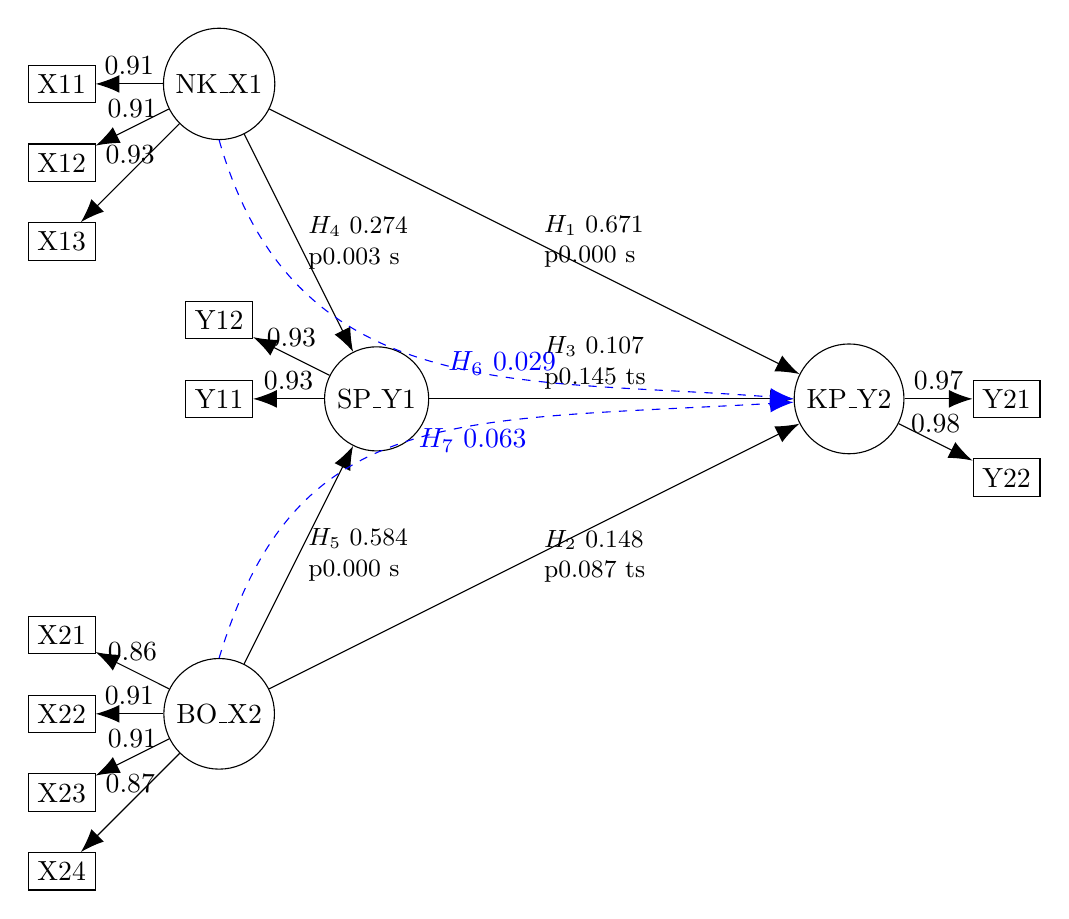
\begin{tikzpicture}
   
    \node (NK_X1)  [draw, circle] at (1,9) {NK\_X1};
    \node (SP_Y1)  [draw, circle] at (3,5) {SP\_Y1};
    \node (BO_X2)  [draw, circle] at (1,1) {BO\_X2};
    \node (KP_Y2)  [draw, circle] at (9,5) {KP\_Y2};


    \node (X21) [draw, rectangle, left of=BO_X2, xshift=-1cm,yshift=1cm] {X21};
    \node (X22) [draw, rectangle, below of=X21] {X22};
    \node (X23) [draw, rectangle, below of=X22] {X23};
    \node (X24) [draw, rectangle, below of=X23] {X24};

    \draw [-{Latex[length=3mm]}] (BO_X2) -- node[above] {0.86} (X21);
    \draw [-{Latex[length=3mm]}] (BO_X2) -- node[above] {0.91} (X22);
    \draw [-{Latex[length=3mm]}] (BO_X2) -- node[above] {0.91} (X23);
    \draw [-{Latex[length=3mm]}] (BO_X2) -- node[above] {0.87} (X24);

    \node (X11) [draw, rectangle, left of=NK_X1,xshift=-1cm] {X11};
    \node (X12) [draw, rectangle, below of=X11] {X12};
    \node (X13) [draw, rectangle, below of=X12] {X13};

    \draw [-{Latex[length=3mm]}] (NK_X1) -- node[above] {0.91} (X11);
    \draw [-{Latex[length=3mm]}] (NK_X1) -- node[above] {0.91} (X12);
    \draw [-{Latex[length=3mm]}] (NK_X1) -- node[above] {0.93} (X13);

    \node (Y11) [draw, rectangle, left of=SP_Y1, xshift=-1cm] {Y11};
    \node (Y12) [draw, rectangle, above of=Y11] {Y12};

    \draw [-{Latex[length=3mm]}] (SP_Y1) -- node[above] {0.93} (Y11);
    \draw [-{Latex[length=3mm]}] (SP_Y1) -- node[above] {0.93} (Y12);

    
    \node (Y21) [draw, rectangle, right of=KP_Y2, xshift=1cm] {Y21};
    \node (Y22) [draw, rectangle, below of=Y21] {Y22};

    \draw [-{Latex[length=3mm]}] (KP_Y2) -- node[above] {0.97} (Y21);
    \draw [-{Latex[length=3mm]}] (KP_Y2) -- node[above] {0.98} (Y22);

    \draw [-{Latex[length=3mm]}] (BO_X2) -- node[right,text width=1.7cm, font=\small] {$H_5$ 0.584 p0.000 s} (SP_Y1);
    \draw [-{Latex[length=3mm]}] (BO_X2) -- node[right,text width=1.7cm, font=\small] {$H_2$ 0.148 p0.087 ts} (KP_Y2);
    \draw [-{Latex[length=3mm]}] (NK_X1) -- node[right,text width=1.7cm, font=\small] {$H_4$ 0.274 p0.003 s} (SP_Y1);
    \draw [-{Latex[length=3mm]}] (NK_X1) -- node[right,text width=1.7cm, font=\small] {$H_1$ 0.671 p0.000 s} (KP_Y2);
    \draw [-{Latex[length=3mm]}] (SP_Y1) -- node[above,text width=1.7cm, font=\small] {$H_3$ 0.107 p0.145 ts} (KP_Y2);

    % \draw [-{Latex[length=3mm]},blue,dashed] (NK_X1) to [bend right=20] node[right] {0.04} (KP_Y2);
    % \draw [-{Latex[length=3mm]},blue,dashed] (BO_X2) to [bend left=20] node[right] {0.07} (KP_Y2);

    \draw [-{Latex[length=3mm]},blue,dashed] (NK_X1.south) .. controls (2,4.8) and (5,5.3) .. node[right] {$H_6$ 0.029} (KP_Y2.west);
    \draw [-{Latex[length=3mm]},blue,dashed] (BO_X2.north) .. controls (2,5) and (4,4.7) ..  node[right] {$H_7$ 0.063} (KP_Y2);
    % \draw [-{Latex[length=3mm]},blue,dashed] (NK_X1) to [bend right=20] node[right] {0.04} (KP_Y2);


\end{tikzpicture}


\end{document}